% This file was created with tikzplotlib v0.10.1.
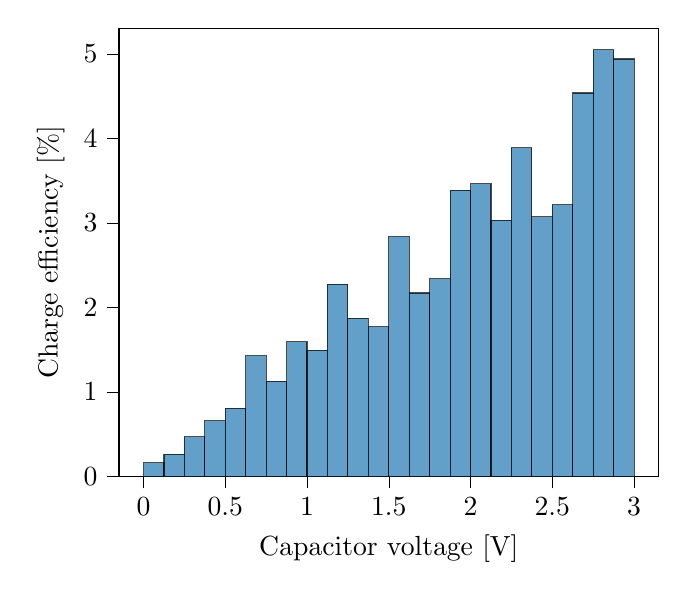
\begin{tikzpicture}

\definecolor{darkgray176}{RGB}{176,176,176}
\definecolor{steelblue31119180}{RGB}{31,119,180}

\begin{axis}[
tick align=outside,
tick pos=left,
x grid style={darkgray176},
xlabel={Capacitor voltage [V]},
xmin=-0.15, xmax=3.15,
xtick style={color=black},
y grid style={darkgray176},
ylabel={Charge efficiency [\%]},
ymin=0, ymax=5.30244997035528,
ytick style={color=black}
]
\draw[draw=black,fill=steelblue31119180,opacity=0.7] (axis cs:0,0) rectangle (axis cs:0.125,0.165231179293843);
\draw[draw=black,fill=steelblue31119180,opacity=0.7] (axis cs:0.125,0) rectangle (axis cs:0.25,0.26353809548904);
\draw[draw=black,fill=steelblue31119180,opacity=0.7] (axis cs:0.25,0) rectangle (axis cs:0.375,0.47215399416917);
\draw[draw=black,fill=steelblue31119180,opacity=0.7] (axis cs:0.375,0) rectangle (axis cs:0.5,0.66153981450183);
\draw[draw=black,fill=steelblue31119180,opacity=0.7] (axis cs:0.5,0) rectangle (axis cs:0.625,0.805974591910235);
\draw[draw=black,fill=steelblue31119180,opacity=0.7] (axis cs:0.625,0) rectangle (axis cs:0.75,1.43154866666915);
\draw[draw=black,fill=steelblue31119180,opacity=0.7] (axis cs:0.75,0) rectangle (axis cs:0.875,1.12611687678152);
\draw[draw=black,fill=steelblue31119180,opacity=0.7] (axis cs:0.875,0) rectangle (axis cs:1,1.59357941507267);
\draw[draw=black,fill=steelblue31119180,opacity=0.7] (axis cs:1,0) rectangle (axis cs:1.125,1.4955410129455);
\draw[draw=black,fill=steelblue31119180,opacity=0.7] (axis cs:1.125,0) rectangle (axis cs:1.25,2.2765953903973);
\draw[draw=black,fill=steelblue31119180,opacity=0.7] (axis cs:1.25,0) rectangle (axis cs:1.375,1.87178803085552);
\draw[draw=black,fill=steelblue31119180,opacity=0.7] (axis cs:1.375,0) rectangle (axis cs:1.5,1.7737171825286);
\draw[draw=black,fill=steelblue31119180,opacity=0.7] (axis cs:1.5,0) rectangle (axis cs:1.625,2.83654503872603);
\draw[draw=black,fill=steelblue31119180,opacity=0.7] (axis cs:1.625,0) rectangle (axis cs:1.75,2.17113744057959);
\draw[draw=black,fill=steelblue31119180,opacity=0.7] (axis cs:1.75,0) rectangle (axis cs:1.875,2.34080557816234);
\draw[draw=black,fill=steelblue31119180,opacity=0.7] (axis cs:1.875,0) rectangle (axis cs:2,3.38604142280018);
\draw[draw=black,fill=steelblue31119180,opacity=0.7] (axis cs:2,0) rectangle (axis cs:2.125,3.46420803076575);
\draw[draw=black,fill=steelblue31119180,opacity=0.7] (axis cs:2.125,0) rectangle (axis cs:2.25,3.03279042140799);
\draw[draw=black,fill=steelblue31119180,opacity=0.7] (axis cs:2.25,0) rectangle (axis cs:2.375,3.88655412321936);
\draw[draw=black,fill=steelblue31119180,opacity=0.7] (axis cs:2.375,0) rectangle (axis cs:2.5,3.07190166264281);
\draw[draw=black,fill=steelblue31119180,opacity=0.7] (axis cs:2.5,0) rectangle (axis cs:2.625,3.21617501075532);
\draw[draw=black,fill=steelblue31119180,opacity=0.7] (axis cs:2.625,0) rectangle (axis cs:2.75,4.53587287583249);
\draw[draw=black,fill=steelblue31119180,opacity=0.7] (axis cs:2.75,0) rectangle (axis cs:2.875,5.04995235271931);
\draw[draw=black,fill=steelblue31119180,opacity=0.7] (axis cs:2.875,0) rectangle (axis cs:3,4.93817986492676);
\end{axis}

\end{tikzpicture}
